%% actual thesis slides


\begin{frame}
\begin{center}
\vspace*{\vfill}
\texttt{\large Thesis title:}\\
\texttt{\Huge Increasing sensitivity to FRBs through ML}
\vspace*{\vfill}
\end{center}
\end{frame}

\begin{frame}{Why?}
\begin{itemize}
		\item Currently applying cuts: 
		\begin{align}
			{\rm S/N} &\geq 8.5 \\
			{\rm DM}  &\geq 50 {\rm pc/cc} \\
			{\rm Width} &\geq 10 {\rm ms}
		\end{align} $\implies$ trigger-rate $\approx 13/$hr.
		\item Reducing S/N would significantly increase the trigger rate.
		\item False positives waste: \begin{itemize}
			\item Disk space on SSD
			\item CPU, human time
			\item Strain on triggering system
				%% system could have worked on other trigger
		\end{itemize}
	\item Machine Learning (ML) as next step in searching.
\end{itemize}
\end{frame}

\begin{frame}{How?}
\begin{itemize}
	\item Input  := Dispersed filterbank chuck
	\item Output := Decision
	\item Required constraints: 
		\begin{description}
		\item[Fast] Realtime capability
		\item[Throughput] Handle Radio Frequency Interference (RFI) strikes
		\item[$\leq$Moderate-weight] Not be computationally demanding
		\end{description}
	\item \emph{A fast ML solution capable of running realtime.}
\end{itemize}
\end{frame}

\subsection{Feature engineering}
\begin{frame}{Bowtie}
	\begin{figure}
	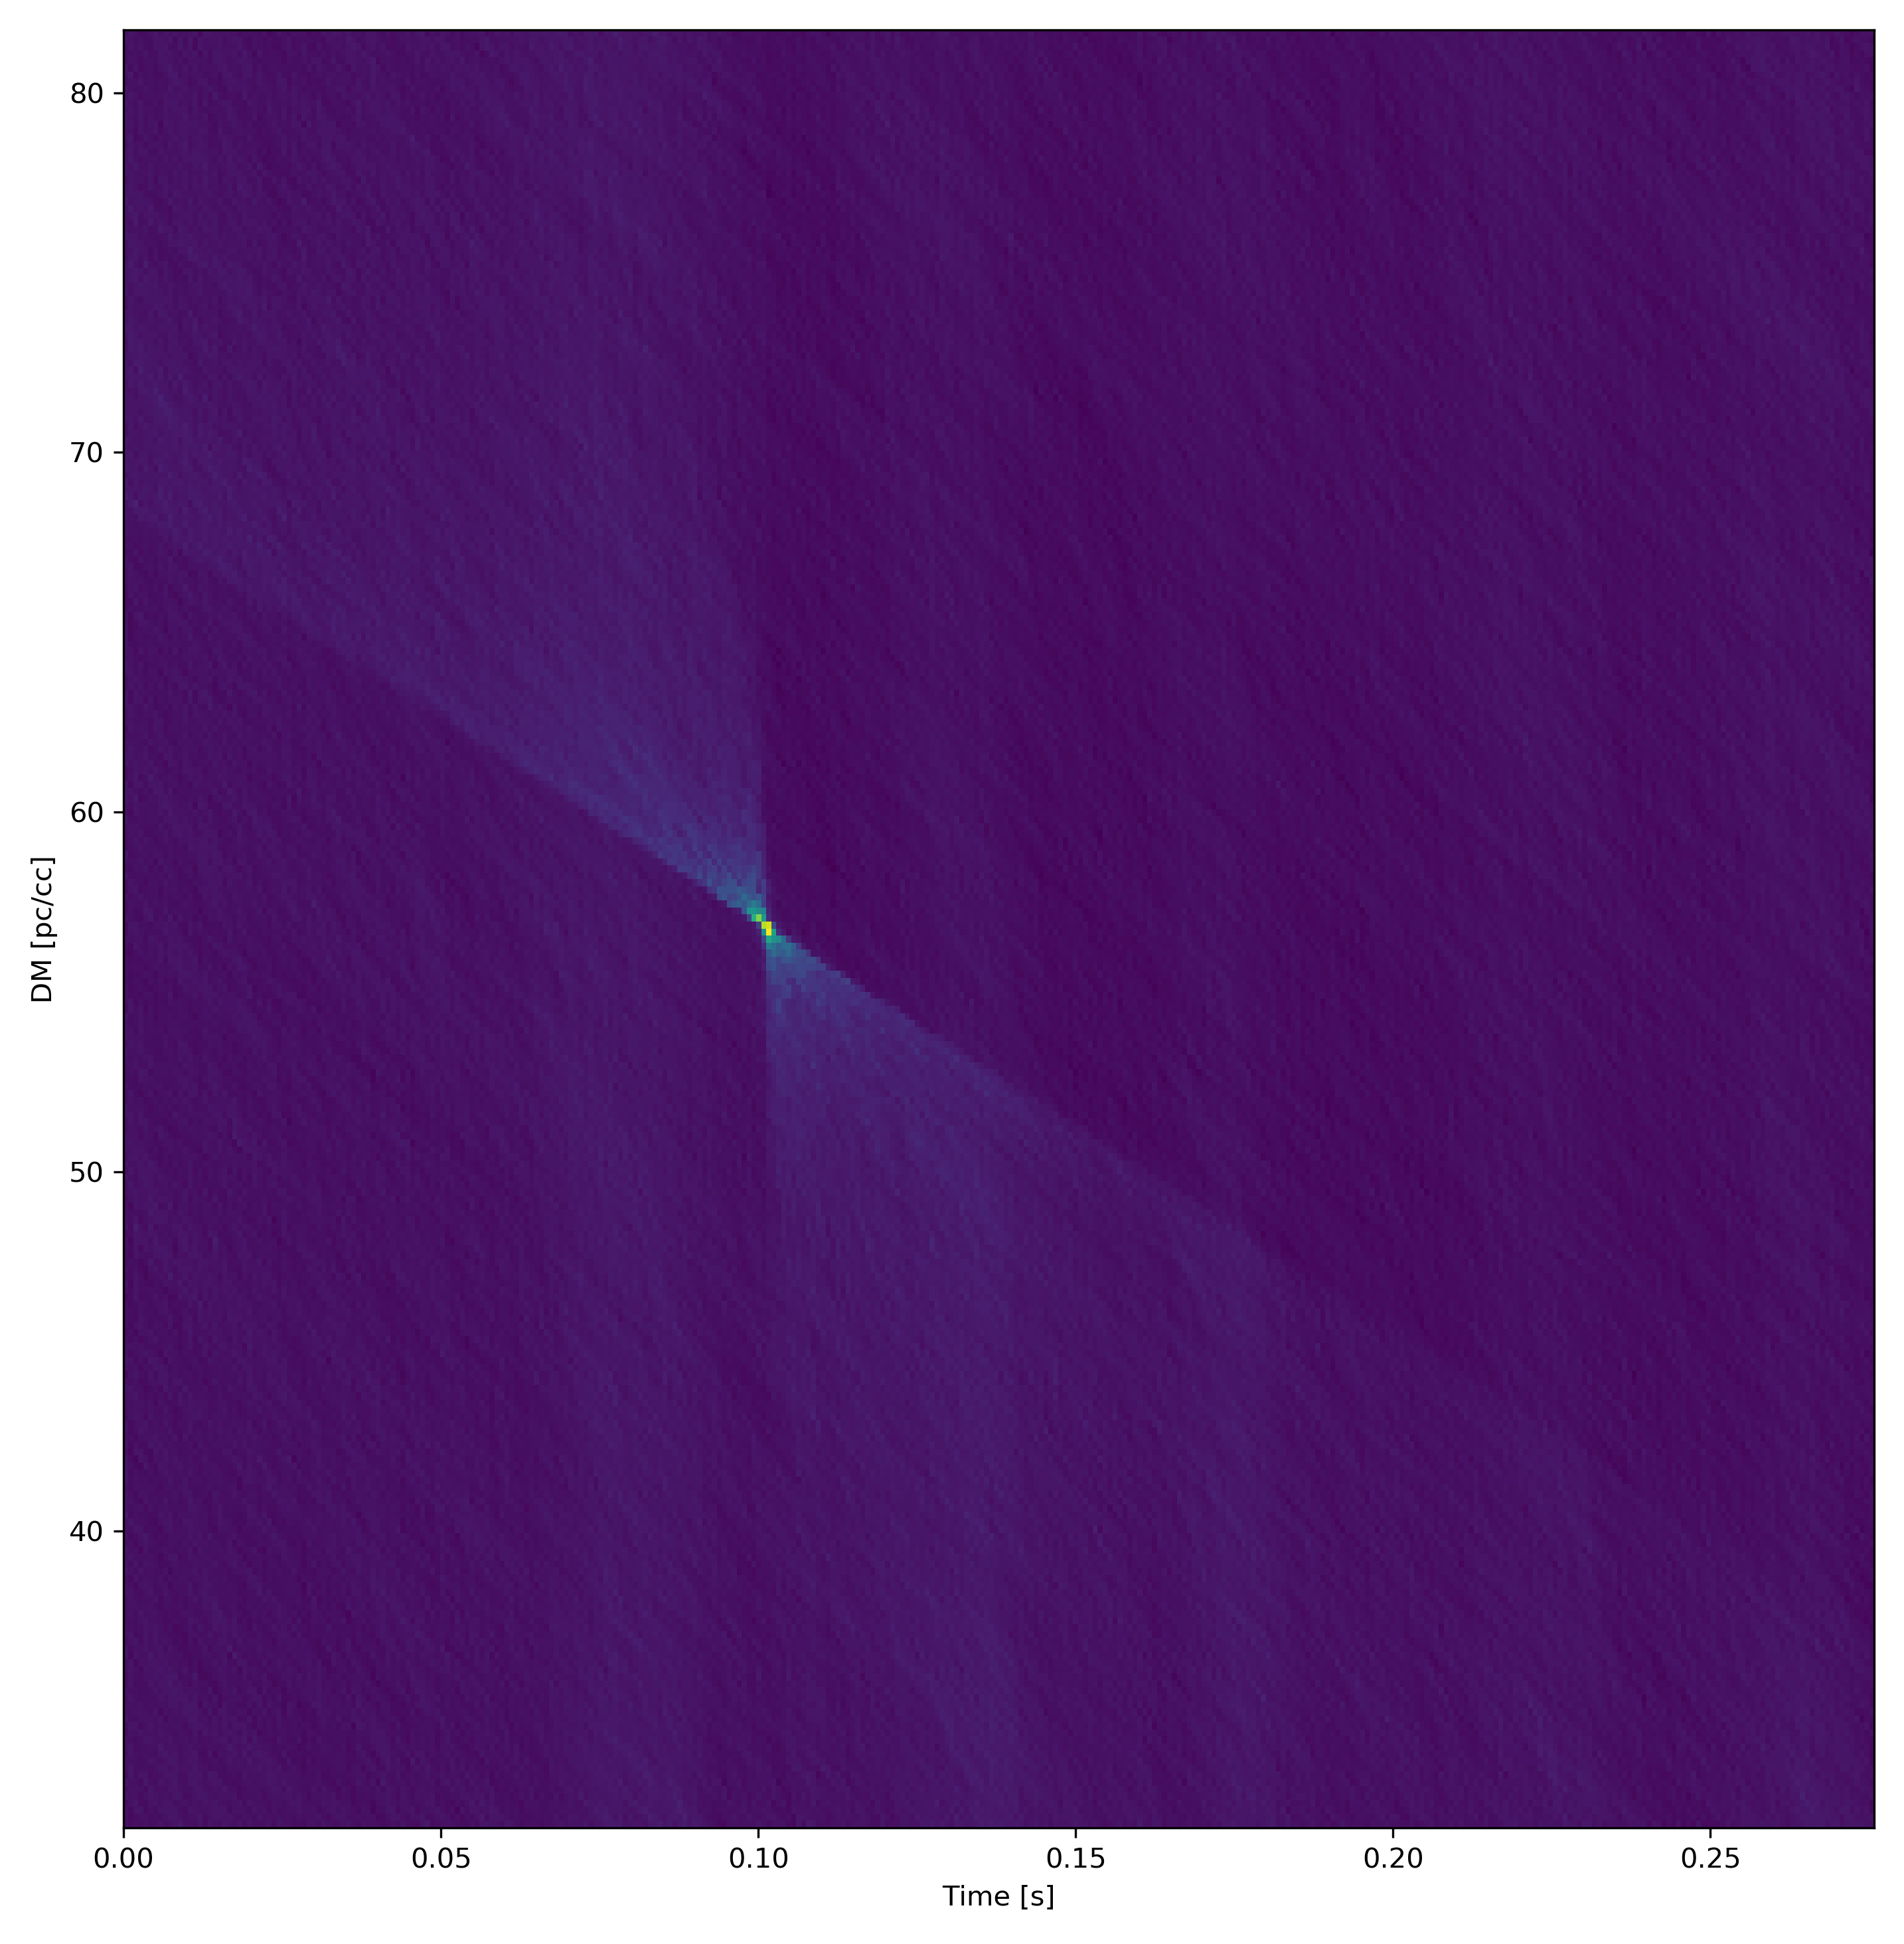
\includegraphics[width=\textwidth,keepaspectratio]{bt_flat.png}
	\label{fig:bt_flat}
	\caption{Offsource ping from Crab psr. S/N=106.58 \emph{(highest)}}
	\end{figure}
\end{frame}

\begin{frame}{Candidate plot}
	\begin{figure}
	\includegraphics[width=\textwidth,keepaspectratio]{}
	\label{fig:candplot}
	\end{figure}
\end{frame}

\begin{frame}[allowframebreaks]{Featureset | Lyon features~\cite{lyon}}
\begin{itemize}
	\item First four standardized moments (mean, variance, skewness, and kurtosis) of \begin{itemize}
			\item S/N as a function of time
			\item S/N as a function of DM
		\end{itemize}
	\item $\mathcal{O}(N)$ operation
	\item Bowtie plane: the most computationally expensive.
	\item Fast De-dispersion Measure Transform (FDMT) \hfill \cite{fdmt}
	\item Power of skewness and kurtosis:
		\begin{figure}
			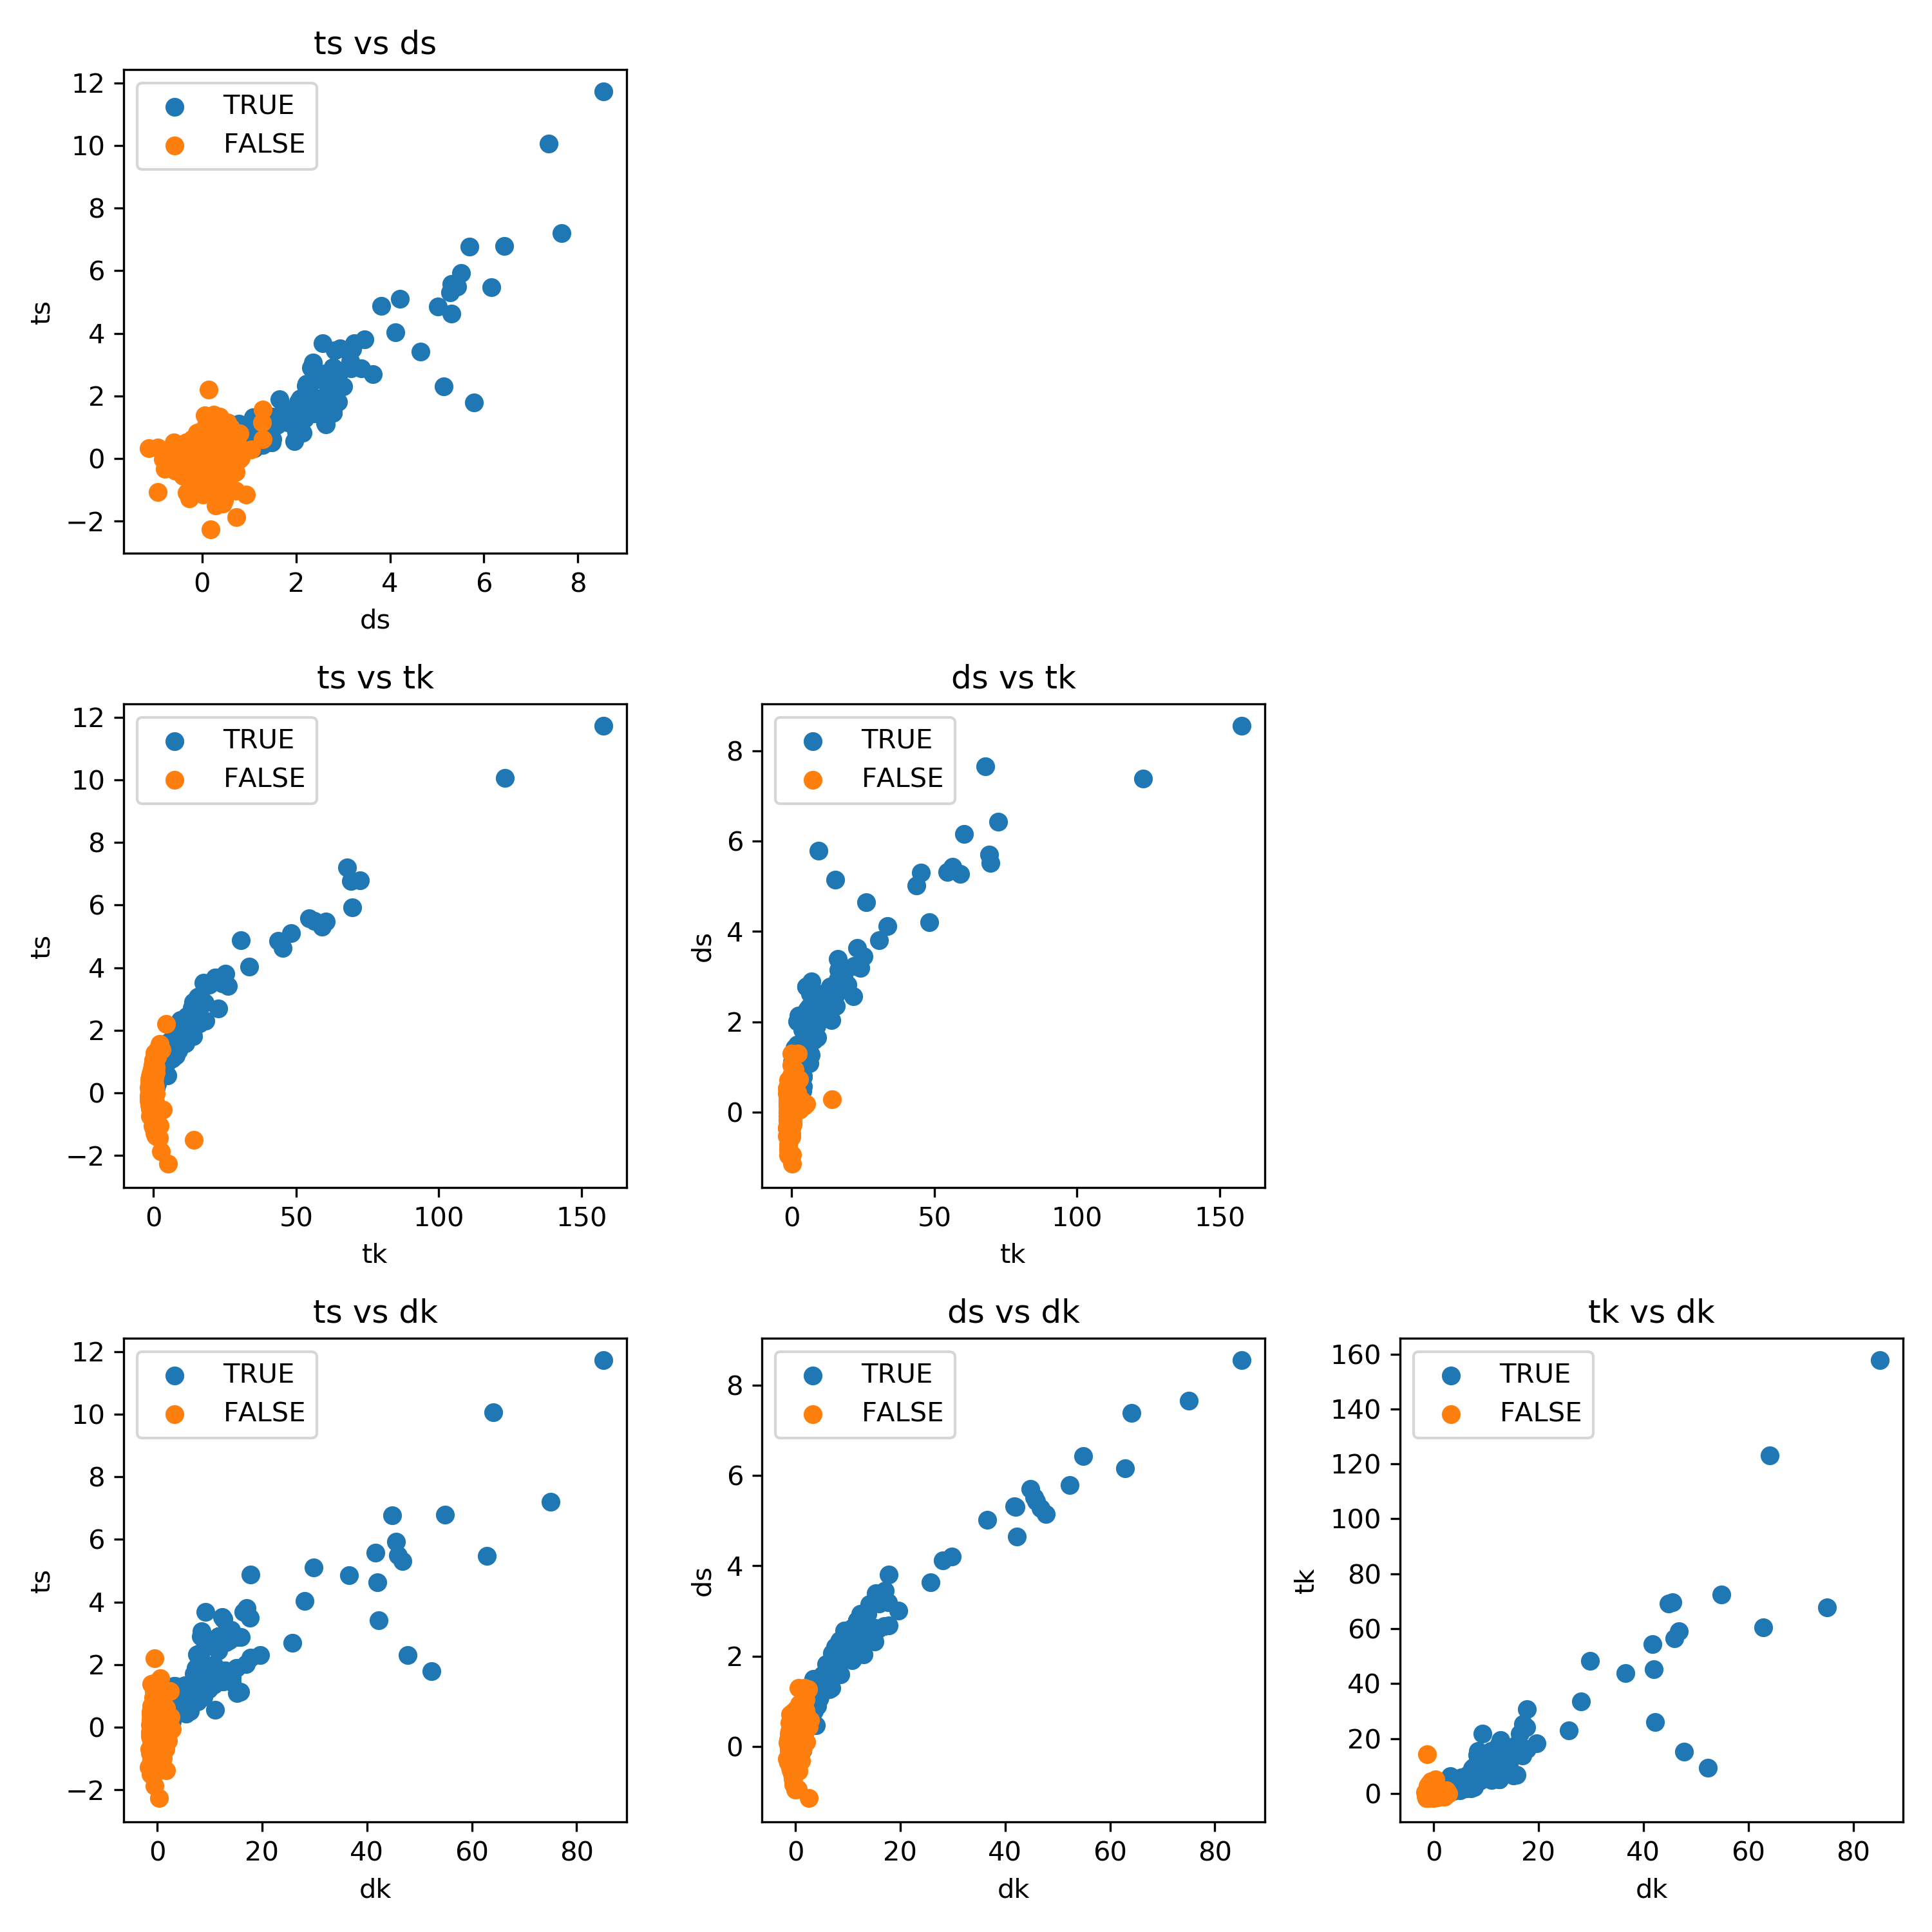
\includegraphics[width=.7\textwidth,keepaspectratio]{corner_td_sk.png}
			\label{fig:corner}
			\caption{Discriminability}
		\end{figure}
\end{itemize}
\end{frame}

\begin{frame}{Still a long way!}
\begin{itemize}
	\item 
\end{itemize}
\end{frame}
